% Mirror: https://github.com/SIGma-UIUC/presentation-format
% --------------------------------------------------------------------
% This is a simple Beamer document that uses beamerthemesigma.sty
% Reading the comments should help you create a presentation even if
% you've never used Beamer before.
% --------------------------------------------------------------------

% Set our document class to Beamer
\documentclass[aspectratio=169]{beamer}
% \documentclass[aspectratio=169, handout]{beamer}
% Add handout option to ignore pauses

% From Jeff E
\usepackage{algo}
% Some more macros
\usepackage{sigmastyle}
% Diagrams
\usepackage{tikz}
\usepackage{minted}
\usetikzlibrary{matrix}

% Set a title
\title{Fast Inverse Square Root}

% Set a subtitle if you desire
\subtitle{}

% Whoever worked on the presentation:
\author{Hassam Uddin}

% Date looks ugly, so leave blank
\date{}

% An institute name, if you're so inclined
% \institute{University of Illinois Urbana-Champaign}

% Use the SIGma theme for this Beamer presentation
\usetheme{sigma}
% --------------------------------------------------------------------

% Begin document
\begin{document}

% Beamer calls each slide a "frame", defined within the environment:
% \begin{frame}
%   <frame content here>
% \end{frame}

% This frame is just the title.
\begin{frame}
\titlepage
\end{frame}

% A frame with the table of contents.
% This frame's title is "Outline".
\begin{frame}{Outline}
  \tableofcontents
\end{frame}


% Start a section: *sections* (subsections, etc.) are what show up in the TOC.
\section{Representing the Reals}
% Section pages can be printed thus:
\frame{\sectionpage}
% There's a way to automate this, see:
% https://tex.stackexchange.com/questions/178800/creating-sections-each-with-title-pages-in-beamers-slides/178803

\begin{frame}{Bases}
    Usually, we represent numbers using their bases. \pause 
    \begin{itemize}
        \item $(425.91)_{10} = 4 \cdot 10^2 + 2\cdot 10^1 + 5 \cdot 10^0 + 9\cdot10^{-1} + 1\cdot 10^{-2}$ \pause 
        \item $(1011.01)_2 = 1\cdot2^3 + 0\cdot 2^{2} + 1\cdot2^1 + 1\cdot2^0 + 0\cdot 2^{-1} + 1 \cdot 2^{-2} = (11.25)_{10}$ \pause 
    \end{itemize}

    In a computer, this has some downsides though. 
\end{frame}


\begin{frame}{Fixed-Point Representations}
    Say we had a fixed 32 bits to represent a decimal number. What are our options? \pause 
    \\
    A few choices: \pause 
    \begin{itemize}
        \item 16 bits for the integer portion, 16 bits for the decimal portion. This means we can only represent up to $65535$, but have a precision of $\approx 1.5 \cdot 10^{-5}$ \pause 
        \item 24 bits for the integer portion, 8 for the decimal? We can go up to $16777215$, but our precision is only $\approx 0.004$. \pause   
    \end{itemize}
    None of these are particularly ideal, we are either severely limiting the largest number we can represent, or the smallest magnitude of precision we have. 
\end{frame}

\begin{frame}{Floating Point Representations}
    Floating point representations are quite similar to scientific notation. \pause
    \begin{itemize}
        \item We can represent $37.56$ as $3.756 \cdot 10^{1}$. \pause
        \item We can represent $(1011.011)_2$ as $1.011011 \cdot 2^{3}$. \pause 
        \item A nice property of binary is that the first bit of a number in this scientific notation will \textit{always} be $1$. \pause
        \item We represent a floating point number $x$ as $\pm q \cdot 2^m$, where $m$ is the exponent, and $q$ is the ``significand'' of the form $1.f$. We refer to $f$ as the fraction, or mantissa.  
    \end{itemize}
\end{frame}

\begin{frame}{Floating Point Representations}
    Our range of representations is much larger, but we aren't as precise. \pause  
    \begin{itemize}
        \item Consider for example $m \in [-4, 4]$ with two bits of the ``fraction,'' giving us 6 total bits for our representation. What are the smallest and largest values we can represent? 
        \item \textbf{NOTE}: For simplicity, although we can represent 15 values with 4 bits in the exponent, we're limiting it to 8 (between -4 and 4). \pause
        \item $x = 1.b_1b_2 \cdot 2^{m}$: Smallest is $(1.00)_2^{-4} = 0.0625$, and the largest is $(1.11)_2 \cdot 2^4 = 28$. \pause  
        \item We can represent much larger values with the same number of bits as a fixed-point, regardless of how we split the fixed-point, while still being able to represent smaller values as well. The only downside is, we're not as precise. How do we represent $27.0$? \pause  
    \end{itemize}
    We cannot represent 27, we're stuck approximating it as $28$ or $24$. 
\end{frame}

\begin{frame}{IEEE-754 Single Precision}
    \begin{figure}
        \centering
        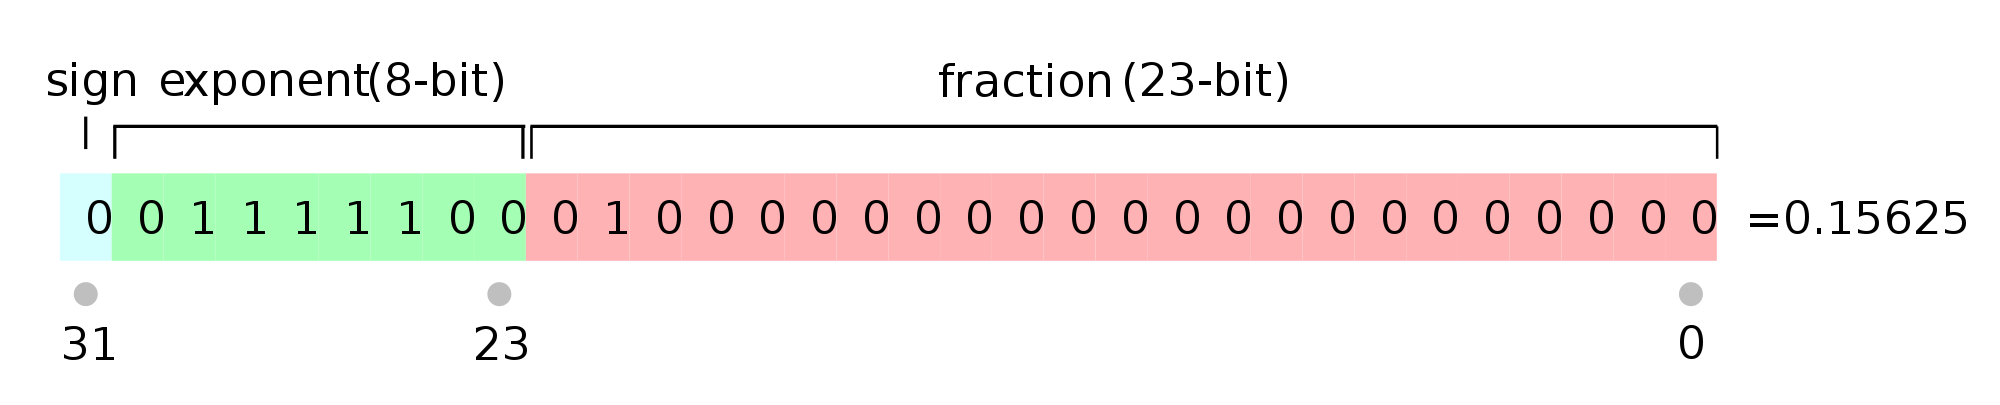
\includegraphics[width=\textwidth]{ieee_single.png}
        \caption{\st{Stolen} Borrowed from CS 357 Notes}
    \end{figure}

    IEEE-754 is \textit{very} similar to a floating point representation but with a few tweaks. 
    $$x = (-1)^s 1.f \cdot 2^m$$
\end{frame}

\begin{frame}{Down to the bits}
    \begin{figure}
        \centering
        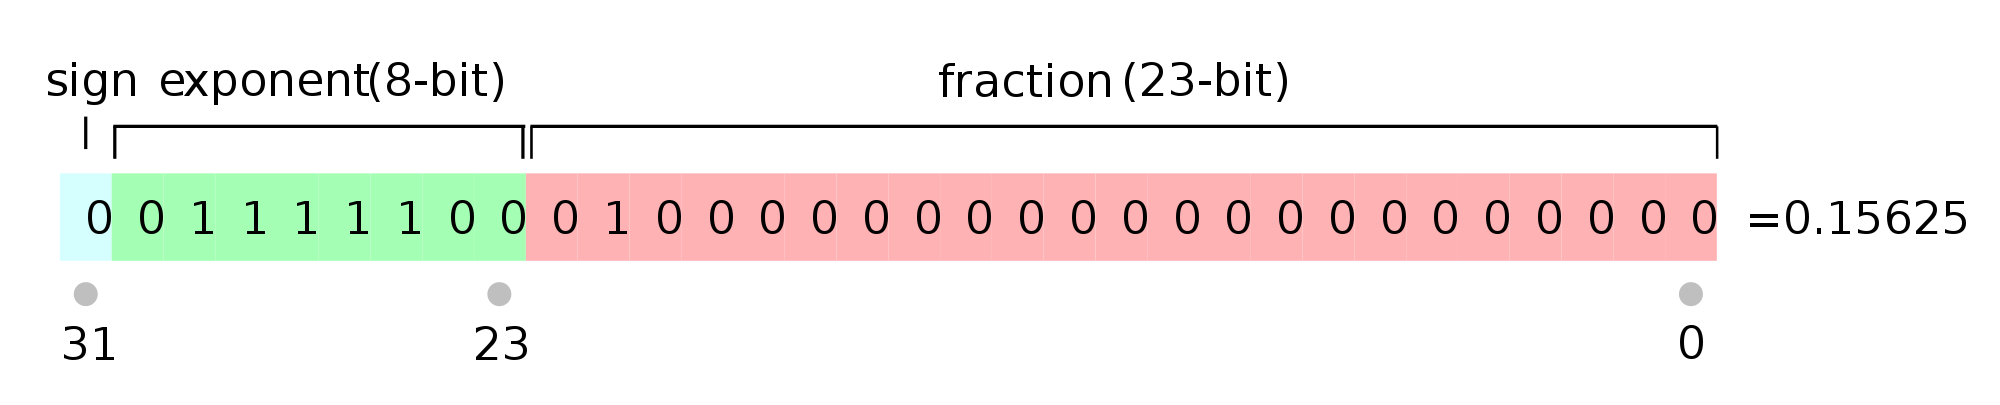
\includegraphics[width=\textwidth]{ieee_single.png}
    \end{figure}
    \begin{itemize}
        \item We use 1 bit for the sign, $s$, leaving us 31 bits. 
        \item We use 8 bits for the exponent, giving us 255 possible exponents. We write $m = c - 127$, where $c$ is the actual exponent stored in the binary representation. We also reserve $c = 0$ and $c = 255$ for special cases. The largest exponent is $127$ and the smallest exponent is $-126$. 
        \item The remaining 23 bits are the fractional part, also known as the mantissa. 
    \end{itemize}
    $$x = (-1)^s 1.f \cdot 2^m$$
\end{frame}

\begin{frame}{Special Cases}
    \begin{itemize}
        \item Zero? \pause We make all the bits in the exponent and the mantissa, or fraction, $0$ to represent 0. Since we don't impact the sign, this means that floats can be $-0$ or $+0$. \pause 
        \item Infinity? \pause If a number is outside our range, we store it as infinity, which we represent as $255$ in the exponent, or by setting all the bits to $1$. We leave the mantissa set to all $0$s. \pause 
        \item NaN? \pause We set all $1$s in the exponent again, but make the mantissa non-zero.
    \end{itemize}

    Rounding values is an important consideration in most cases, take CS 357 (or just watch the two lectures associated with floating point numbers) to understand how we use floating points and how we should be careful with them. 
\end{frame}

\begin{frame}{Matching bits}
    What happens if we take the bits in a floating point number and just ``pretend'' that it's an integer? What if we do the opposite? \pause 
    
    Let us ignore the sign bit for a moment: $x = 1.f \cdot 2^{c - 127}$. Reinterpreting these bits as an integer, we get $x_{int} = c \cdot 2^{23} + f$.  \pause

    Converting an integer to a float is less clean, so I'll leave that to you. 

\end{frame}

\section{Abusing IEEE-754 for fun and profit}
\frame{\sectionpage}

\begin{frame}{Fast Logarithms}
    \begin{itemize}
        \item Let's take the logarithm of our float representation. \pause
        \item If we consider the mantissa and the exponent as integers, we can write $x_{float} = (1 + \frac{f}{2^{23}}) \cdot 2^{c - 127}$. If we take the logarithm of this: 
            $$ \log_2 ((1 + \frac{f}{2^{23}}) \cdot 2^{c - 127}) = \log_2(1 + \frac{f}{2^{23}}) + c - 127$$
        \pause 
        \item Recall that we can approximate $\log(1 + x) \approx \log(x)$, and we can add an error correction factor $\mu$, to make our approximation even tighter. \pause 
        \item So our log is now:
        $$ \frac{f}{2^{23}} + \mu + c - 127 = \frac{1}{2^{23}}(f + c \cdot 2^{23}) + \mu - 127$$ 
    \end{itemize}
\end{frame}

\begin{frame}{Hmm}
\begin{itemize}
    \item Something suspicious has appeared. Our logarithm is of the form $k_1(f + c \cdot 2^{23}) + k_2$, where $k_1$ and $k_2$ are constants. \pause 
    

    \item Recall, however, that the integer reinterpretation of our floating point number is $f + c \cdot 2^{23}$. \pause 

    \item We can approximate $\log_2(x_{float})$ as a linear transformation of $x_{int}$. No computation needed! \pause  

    \item How easy would it be to go from $\log_2(x_{float})$ back to the regular number? \pause

    \item We just undo the linear transform: we've gotten all the log properties for free!
\end{itemize}
\end{frame}

\begin{frame}{Square root a log-approximated number}
    \begin{itemize}
        \item Let's take the square root of $x_{float}$ by abusing these properties. \pause 
        \item First, recall that $k\log(x) = \log(x^k)$, so $x_{float}^{1/2} = 2^{1/2 \cdot \log_2(x_{float})}$. \pause 
        \item So, we can compute $2^{1/2 \cdot (k_1x_{int} + k_2)}$ \pause 
        \item How do we find our constants $k_1, k_2$, and do this computation quickly? \pause 
        \item Let's detour into taking the \textit{inverse} square root
    \end{itemize}
\end{frame}

\section{Quake's Fast Inverse-Square-Root}
\frame{\sectionpage}

\usemintedstyle{borland}
\begin{frame}[containsverbatim]{A detour into history}
\begin{minted}
[
baselinestretch=0.6,
]
{c}
float q_rsqrt(float number)
{
  long i;
  float x2, y;
  const float threehalfs = 1.5F;

  x2 = number * 0.5F;
  y  = number;
  i  = * ( long * ) &y; // evil floating point bit level hacking
  i  = 0x5f3759df - ( i >> 1 ); // what the fuck?
  y  = * ( float * ) &i;
  y  = y * ( threehalfs - ( x2 * y * y ) ); // 1st iteration
  // y  = y * ( threehalfs - ( x2 * y * y ) ); // 2nd iteration, this can be removed

  return y;
}
    \end{minted}
\end{frame}

\begin{frame}[containsverbatim]{Modernize}
\begin{minted}
[
baselinestretch=0.6
]
{c++}
constexpr float Q_rsqrt(float number) noexcept
{
  // only allow on IEEE-754 floats
  static_assert(std::numeric_limits<float>::is_iec559);

  // what the fuck? (left for historical accuracy)
  // make use of std::bit_cast to avoid undefined behavior
  float const y = std::bit_cast<float>(
    0x5f3759df - (std::bit_cast<std::uint32_t>(number) >> 1));
  return y * (1.5f - (number * 0.5f * y * y));
}
\end{minted}
\end{frame}

\begin{frame}[containsverbatim]{evil floating point bit level hacking}
\begin{minted}
[
baselinestretch=0.6,
linenos=false
]
{c}
i = * ( long * ) &y;     
\end{minted}
or
\begin{minted}
[
baselinestretch=0.6,
linenos=false
]
{c++}
std::bit_cast<std::uint32_t>(number)   
\end{minted}
\pause 

This reinterprets the floating point number as an integer. 

\end{frame}

\begin{frame}[fragile]{what the fuck?}
    \begin{minted}
[
baselinestretch=0.6,
linenos=false
]
{c}
i  = 0x5f3759df - ( i >> 1 );  
\end{minted}
\pause 

\begin{itemize}
    \item Recall that $-\frac{1}{2} \log(y) = \log(\frac{1}{\sqrt{y}})$ \pause 
    \item Call $\frac{1}{\sqrt{y}} = Y$, and let us substitute the bit representation of each in place of their log: \pause
    $$\frac{1}{2^{23}} (f_{Y} + c_{Y} \cdot 2^{23}) + \mu - 127 = -\frac{1}{2}\left(\frac{1}{2^{23}} (f_{y} + c_{y} \cdot 2^{23}) + \mu - 127\right)$$
    \item Let's solve for the bit representation of $Y$: $f_{Y} + c_Y \cdot 2^{23}$: \pause 
    $$ f_{Y} + c_{Y} \cdot 2^{23} = \frac{3}{2} 2^{23}(127 - \mu) - \frac{1}{2}(f_y + c_y \cdot 2^{23}) $$
\end{itemize}
\end{frame}

\begin{frame}[fragile]{0x5f3759df?}
\begin{overprint}
\onslide<1>
\begin{minted}
[
baselinestretch=0.6,
linenos=false,
escapeinside=||
]
{c}
i  = 0x5f3759df - ( i >> 1 );  
\end{minted}
\onslide<2->
\begin{minted}
[
baselinestretch=0.6,
linenos=false,
escapeinside=||
]
{c}
i  = 0x5f3759df - |\color{red}( i >> 1 )|;  
\end{minted}

\end{overprint}
$$ f_{Y} + c_{Y} \cdot 2^{23} = {\only<3->{\color{blue}} \frac{3}{2} 2^{23}(127 - \mu)} - {\only<2->{\color{red}}\frac{1}{2}(f_y + c_y \cdot 2^{23})} $$

\begin{itemize}
    \item \onslide<4-> How did we choose the ``magic constant'' $\mu$?
    \item \onslide<5-> Historically, it's unknown, and the choice of constant used in Quake is actually not optimal. 
    \item \onslide<6-> If you were doing this in your own program, plot the error and minimize. 
\end{itemize}

\end{frame}

\begin{frame}[fragile]{Casting back}
\begin{minted}
[
baselinestretch=0.6,
linenos=false
]
{c}
y  = * ( float * ) &i;
\end{minted}

or 
\begin{minted}
[
baselinestretch=0.6,
linenos=false
]
{c++}
float const y = std::bit_cast<float>(...);
\end{minted}

\pause 
\begin{itemize}
    \item Are we done? \pause 
    \item We are quite close, but we've introduced a decent amount of error in our assumptions. 
\end{itemize}
\end{frame}

\begin{frame}{Newton's Method, another detour}
    The goal: find $c$ such that $f(c) = 0$\pause 
    \begin{itemize}
        \item We want to make a guess that is close to $c$ \pause 
        \item Find the tangent line and solve for its $0$: $0 = f(x_0) + f'(x_0)(x_1 - x_0) \implies x_1 = x_0 - \frac{f(x_0)}{f'(x_0)}$ \pause
        \item Repeat until we're happy \pause 
    \end{itemize}
    \begin{figure}
        \centering
        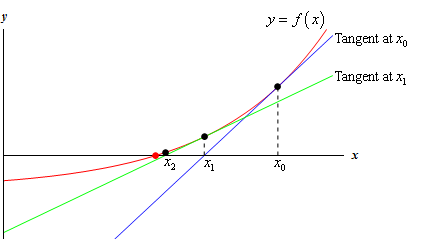
\includegraphics[width=0.5\textwidth]{image001.png}
        \caption{Paul's Math Notes}
    \end{figure}
\end{frame}

\begin{frame}{Newton's method, on inverse square root}
    \begin{itemize}
        \item We want to find $\frac{1}{\sqrt{x}}$, so minimize $\text{error}(y) = \frac{1}{y^2} - x$
        \item Plugging into Newton's method, we have: 
        $$y_1 = y_0 - \frac{y_0^{-2} - x}{-2y_0^{-3}} = \frac{1}{2}y_0(3 - xy_0^2)$$
    \end{itemize}
\end{frame}

\begin{frame}[fragile]{Another look}
$$\frac{1}{2}y_0(3 - xy_0^2)$$
\begin{minted}
[
baselinestretch=0.6
]
{c++}
constexpr float Q_rsqrt(float number) noexcept
{
  // only allow on IEEE-754 floats
  static_assert(std::numeric_limits<float>::is_iec559);

  // what the fuck? (left for historical accuracy)
  // make use of std::bit_cast to avoid undefined behavior
  float const y = std::bit_cast<float>(
    0x5f3759df - (std::bit_cast<std::uint32_t>(number) >> 1));
  return y * (1.5f - (number * 0.5f * y * y));
}
\end{minted}
\end{frame}

\begin{frame}{Does the fun stop here?}
    \begin{itemize}
        \item The inverse square root does not have any divisions, so it is ``fast.'' \pause 
        \item Quake uses this for the inverse square root because taking the inverse square root of a vector's length is a common operation to normalize a vector. \pause 
        \item We can approximate a \textit{lot} of functions using this approach while avoiding any divisions. 
    \end{itemize}
\end{frame}

\begin{frame}{ECE Majors strike again}
    \begin{itemize}
        \item Unfortunately, we're not allowed to have fun in a world with hardware engineers. \pause 
        \item Intel SSE (found on any computer made after 1999), has the RSQRTSS instruction. \pause 
    \end{itemize}
    
    \begin{figure}
    \centering
    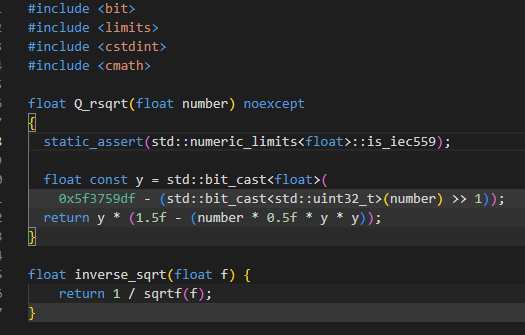
\includegraphics[width=0.49\linewidth]{image.png}
    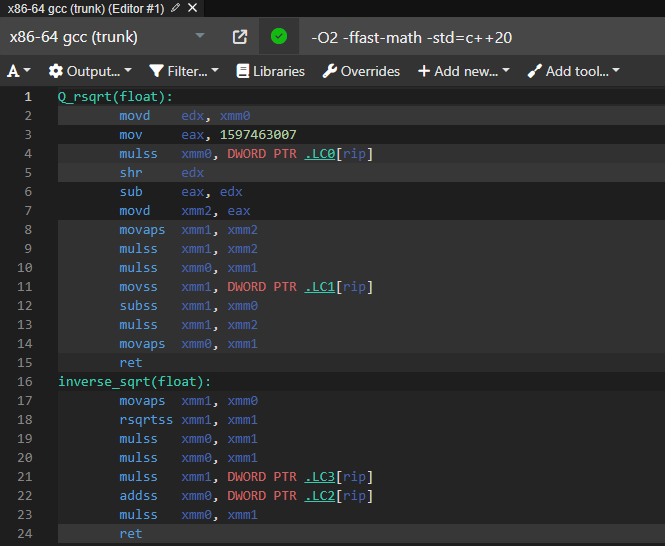
\includegraphics[width=0.49\linewidth]{assembly.png}
\end{figure}
\end{frame}

\begin{frame}{All is not lost}
    \begin{itemize}
        \item Inverse square root is such a common operation that it is built into modern hardware \pause 
        \item But, keep in mind, when you're doing any computation, logs and powers are just a cast and linear transformation away. 
    \end{itemize}
\end{frame}

\begin{frame}{}
      \begin{center}
    {\color{sigma@mainblue} \LARGE Questions?}
  \end{center}
\end{frame}


% Quotes are fun, find some to use!
\font\eightss=cmssq8
\font\eightssi=cmssqi8
\newcommand\quoteAuthorDate[3]{\begingroup
  \baselineskip 10pt
  \parfillskip 0pt
  \interlinepenalty 10000 % not needed in example
  \leftskip 0pt plus 40pc minus \parindent
  \let\rm=\eightss
  \let\sl=\eightssi
  \everypar{\sl}#1\par
  \nobreak\smallskip
  \noindent\rm--- #2\unskip\enspace(#3)\par
  \endgroup}
% If someone can figure out how to horizontally center this and make the text bigger that'd be cool
\begin{frame}
    \begin{center}
        \item \quoteAuthorDate{Truth is much too complicated to allow anything but approximations.}{John Von Nuemann}{\textcolor{sigma@mainblue}{1947}}
    \end{center}
\end{frame}

% Remove this slide if you came up with all the material yourself


\end{document}